\documentclass[11pt]{amsart}
\usepackage[english]{babel}
\usepackage{amsmath}
\usepackage{amsfonts}
\usepackage{amssymb}
%\usepackage{showlabels}
\usepackage{amsthm}
\usepackage{marginnote}

\usepackage[english]{babel}
\usepackage{yfonts}
\usepackage[T1]{fontenc}
\usepackage[utf8x]{inputenc}
\usepackage{enumerate}
\usepackage{verbatim}
\usepackage{graphicx}
\usepackage{verbatim}
\usepackage{faktor}
\usepackage{xcolor}
\usepackage{xfrac}
\usepackage{tikz,tikz-cd}
\usepackage[all]{xy}
\usepackage{bbm}

\newcommand{\M}[4]{\overline{\mathcal M}_{#1,#2}(#3,#4)}
\newcommand{\Q}[4]{\overline{\mathcal Q}_{#1,#2}(#3,#4)}
\newcommand{\Qt}[4]{\widetilde{\mathcal Q}_{#1,#2}(#3,#4)}
\newcommand{\PP}{\mathbb P}
\newcommand{\Z}{\mathbb{Z}}
\newcommand{\N}{\mathbb{N}}
\newcommand{\OO}{\mathcal{O}}
\renewcommand{\to}{\rightarrow}
\newcommand{\A}{\mathcal A}
\newcommand{\B}{\mathcal B}
\newcommand{\C}{\mathfrak C}
\renewcommand{\L}{\mathcal L}
\newcommand{\MM}{\mathfrak M}
\newcommand{\Aaff}{\mathbb{A}}
\newcommand{\kfield}{\mathbb{K}}
\newcommand{\comp}{\chi}
\newcommand{\sst}{\sigma^{ss}}
\newcommand{\Pic}{\operatorname{Pic}}
\newcommand{\Def}{\operatorname{Def}}
\newcommand{\Spec}{\operatorname{Spec}}
\newcommand{\Proj}{\operatorname{Proj}}
\newcommand{\Hom}{\operatorname{Hom}}
\newcommand{\Ext}{\operatorname{Ext}}
\newcommand{\Gm}{\mathbb{G}_m}

\newcommand{\bq}{\begin{equation}}
\newcommand{\eq}{\end{equation}}
\newcommand{\ba}{\begin{aligned}}
\newcommand{\ea}{\end{aligned}}
\newcommand{\be}{\begin{enumerate}}
\newcommand{\ee}{\end{enumerate}}
\newcommand{\bsm}{\left(\begin{smallmatrix}}
\newcommand{\esm}{\end{smallmatrix}\right)}                   
\newcommand{\bpm}{\begin{pmatrix}}
\newcommand{\epm}{\end{pmatrix}}
\newcommand{\barr}{\begin{displaymath}\begin{array}{cccc}}
\newcommand{\earr}{\end{array}\end{displaymath}}
\newcommand{\barrl}{\begin{displaymath}\begin{array}{lcl}}
\newcommand{\earrl}{\end{array}\end{displaymath}}
\newcommand{\barl}{\begin{displaymath}\begin{array}{l}}
\newcommand{\earl}{\end{array}\end{displaymath}}
\newcommand{\bxym}{ \begin{displaymath}\xymatrix }
\newcommand{\exym}{\end{displaymath}}
\newcommand{\bcd}{\begin{center}\begin{tikzcd}}
\newcommand{\ecd}{\end{tikzcd}\end{center}}

\newcommand{\tr}{{\rm tr}}
\newcommand{\Isom}{\text{Isom}}
\newcommand{\pr}{\operatorname{pr}}
\newcommand{\ev}{\operatorname{ev}}
\newcommand{\codim}{\operatorname{codim}}
\newcommand{\vdim}{\operatorname{vdim}}
\newcommand{\ildef}[1]{\textbf{\textsc{#1}}}

\theoremstyle{plain}
\newtheorem{thm}{Theorem}[section]
\newtheorem{lem}[thm]{Lemma}
\newtheorem{prop}[thm]{Proposition}
\newtheorem{cor}[thm]{Corollary}
\newtheorem*{teo*}{Theorem}
\newtheorem{ipotesi}{ipotesi}
\newtheorem*{nota}{Nota}
\newtheorem{claim}{Claim}
\newtheorem{question}[thm]{Question}
\newtheorem{conj}[thm]{Conjecture}

\theoremstyle{definition}
\newtheorem{example}[thm]{Example}
\newtheorem{ex}[thm]{Example}
\newtheorem{dfn}[thm]{Definition}
\newtheorem{aside}[thm]{Aside}
\newtheorem{remark}[thm]{Remark}
\newtheorem{com}[thm]{Comment}
\newtheorem{num}{Number}
\newtheorem*{sketch}{Sketch}
\newtheorem*{rem}{Remark}


\newcommand{\todo}[1]{\vspace{5mm}\par \noindent
\framebox{\begin{minipage}[c]{0.95 \textwidth} \tt #1\end{minipage}} \vspace{5mm} \par}

\def\ti{-\allowhyphens}
\newcommand{\thismonth}{\ifcase\month % case 0 --- impossible!
  \or January\or February\or March\or April\or May\or June%
  \or July\or August\or September\or October\or November%
  \or December\fi}
\newcommand{\thismonthyear}{{\thismonth} {\number\year}}
\newcommand{\thisdaymonthyear}{{\number\day} {\thismonth} {\number\year}}

\usepackage[T1]{fontenc}
\usepackage{newpxtext,newpxmath}

\title{Genus 0 Relative Toric Quasimaps \`a la Gathmann}
\author{Luca Battistella and Navid Nabijou}
\begin{document}

\begin{abstract}
Relative quasimaps are good.
\end{abstract}

\maketitle

\section{Functoriality of Quasimap Spaces}

In the case of stable maps, a morphism $f : X \to Y$ induces a morphism between the corresponding moduli spaces
\begin{equation*}\M{g}{n}{X}{\beta} \rightarrow \M{g}{n}{Y}{f_* \beta} \end{equation*}
given by composition with $f$ (in general this induced morphism may involve stabilisation of the source curve). Because of this, the construction of the moduli space of stable maps is said to be \ildef{functorial}.

It is natural to ask whether the same holds for the moduli space of quasimaps. Since here the objects of the moduli space are not maps, we cannot simply compose with $f$, and indeed it is not immediately clear how we should proceed. In \cite[Section 3.1]{CF-K-wallcrossing} a definition is given when $f$ is an embedding into a projective space; however, this uses the more general language of GIT quotients which we seek to avoid here. As such, we will provide an alternative (but entirely equivalent) construction in the setting of toric varieties, which also relaxes the conditions on the map $f$ and the target $Y$.

\footnote{We should probably look a bit harder to see if the definition exists elsewhere.}

Our approach uses the language of $\Sigma$--collections introduced by D. Cox. This approach is natural insofar as a quasimap is a generalisation of a $\Sigma$--collection. We will refer extensively to \cite{CoxRing} and \cite{CoxFunctor}, which we recommend as an  introduction for any readers unfamiliar with the theory.

Let $X$ and $Y$ be smooth and proper toric varieties with fans $\Sigma_X \subseteq N_X$ and $\Sigma_Y \subseteq N_Y$. Suppose we are given $f : Y \to X$ (which we do not assume to be a toric morphism). By \cite[Theorem 1.1]{CoxFunctor} the data of such a map is equivalent to a $\Sigma_X$--collection on $Y$:
\begin{equation*} ( (L_\rho, u_\rho)_{\rho \in \Sigma_X(1)}, (\varphi_{m_x})_{m_x \in M_X} ) \end{equation*}
In addition, \cite{CoxRing} allows us to describe line bundles on $Y$ and their global sections in terms of the homogeneous coordinates $(z_\tau)_{\tau \in \Sigma_Y(1)}$. All of these observations are combined into the following theorem, which is so useful that we will state it here in its entirety:

\begin{thm} \cite[Theorem 2.2]{CoxFunctor} \label{CoxTheorem} The data of a morphism $f:Y \to X$ is the same as the data of homogeneous polynomials
\begin{equation*} P_\rho \in S^Y_{\beta_\rho} \end{equation*}
for $\rho \in \Sigma_X(1)$, where $\beta_\rho \in \Pic Y$ and $S^Y_{\beta_\rho}$ is the corresponding graded piece of the Cox ring
\begin{equation*}S^Y = k[z_\tau : \tau \in \Sigma_Y(1)]\end{equation*}
This data is required to satisfy the following two conditions:
\begin{enumerate}
\item $\sum_{\rho \in \Sigma_X(1)} \beta_\rho \otimes n_\rho = 0$ in $\Pic Y \otimes N_X$.
\item $(P_\rho(z_\tau)) \notin Z(\Sigma_X) \subseteq \Aaff_k^{\Sigma_X(1)}$ whenever $(z_\tau) \notin Z(\Sigma_Y) \subseteq \Aaff_k^{\Sigma_Y(1)}$.
\end{enumerate}
Furthermore, two such sets of data $(P_\rho)$ and $(P^\prime_\rho)$ correspond to the same morphism if and only if there exists a $\lambda \in \Hom_\Z(\Pic X, \Gm)$ such that
\begin{equation*} \lambda(D_\rho) \cdot P_\rho = P^\prime_\rho \end{equation*}
for all $\rho \in \Sigma_X(1)$. Finally, if we define $\tilde{f}(z_\tau) = (P_\rho(z_\tau))$ then this defines a lift of $f$ to the prequotients:
\bcd
\Aaff_k^{\Sigma_Y(1)} \setminus Z(\Sigma_Y) \ar[r, "\tilde{f}"] \ar[d, "\pi"] & \Aaff_k^{\Sigma_X(1)} \setminus Z(\Sigma_X) \ar[d,"\pi"] \\
Y \ar[r, "f"] & X
\ecd
\end{thm}
\begin{aside} Throughout this section we will stick to the notation established above; in particular we will use $\rho$ to denote a ray in $\Sigma_X(1)$ and $\tau$ to denote a ray in $\Sigma_Y(1)$. \end{aside}

Recall our goal: given a map $f : Y \to X$ we wish to define a ``push-forward'' map:
\begin{equation*} f_* : \Q{g}{n}{Y}{\beta} \to \Q{g}{n}{X}{f_*\beta} \end{equation*}
Consider therefore a quasimap $(C, (L_\tau, u_\tau)_{\tau \in \Sigma_Y(1)}, (\varphi_{m_Y})_{m_Y \in M_Y})$ with target $Y$. Pick data $(P_\rho)_{\rho \in \Sigma_X(1)}$ corresponding to the map $f$, as in the theorem above; we will later see that our construction does not depend on this choice.

The idea of the construction is as follows. Let us pretend for a moment that $C$ is toric and that the quasimap is without basepoints, so that we have an actual morphism $C \to Y$. Then we can lift this morphism to the prequotient as in the following diagram

\bcd
\Aaff_k^{\Sigma_C(1)} \setminus Z(\Sigma_C) \ar[r, "(u_\tau)"] \ar[d] & \Aaff_k^{\Sigma_Y(1)} \setminus Z(\Sigma_Y) \ar[r, "(P_\rho)"] \ar[d] & \Aaff_k^{\Sigma_X(1)} \setminus Z(\Sigma_X) \ar[d] \\
C \ar[r] & Y \ar[r] & X
\ecd
from which it follows that the composition $C \to Y \to X$ is given in homogeneous coordinates by:
\begin{equation*} (P_\rho((u_\tau)_{\tau \in \Sigma_Y(1)}))_{\rho \in \Sigma_X(1)} \end{equation*}
In general of course $C$ is not a toric variety and the quasimap is not basepoint-free. Nevertheless, as we will see, we can still make sense of the expression $P_\rho(u_\tau)$ as a section of a line bundle on $C$. This will allow us to define the pushforward of our quasimap.

Let us begin. For each $\rho$, $P_\rho$ is a polynomial in the $z_\tau$; we can write it as
\begin{equation} \label{Prho} P_\rho(z_\tau) = \sum_{\underline{a}} P_\rho^{\underline{a}}(z_\tau) = \sum_{\underline{a}} \mu_{\underline{a}} \prod_{\tau} z_{\tau}^{a_{\tau}} \end{equation}
where the sum is over a finite number of multindices $\underline{a} = (a_\tau) \in \N^{\Sigma_Y(1)}$ and the $\mu_{\underline{a}}$ are nonzero scalars. For each $\underline{a}$ consider the following line bundle on $C$:
\begin{equation*} \tilde{L}_\rho^{\underline{a}} = \bigotimes_\tau L_\tau^{\otimes a_\tau} \end{equation*}
Then we may take the following section of $\tilde{L}_\rho^{\underline{a}}$:
\begin{equation*} \tilde{u}_\rho^{\underline{a}} = P_\rho^{\underline{a}}(u_\tau) = \mu_{\underline{a}} \prod_\tau u_\tau^{a_\tau} \end{equation*}
Thus each of the terms $P_\rho^{\underline{a}}$ of $P_\rho$ defines a section $\tilde{u}_\rho^{\underline{a}}$ of a line bundle $\tilde{L}_\rho^{\underline{a}}$. But what we want is a single section $\tilde{u}_\rho$ of a single line bundle $\tilde{L}_\rho$. This is where the isomorphisms $\varphi_{m_Y}$ come in.

Recall that we have a short exact sequence:
\begin{equation} \label{Pic short exact sequence for Y} 0 \longrightarrow M_Y \overset{\theta}{\longrightarrow} \Z^{\Sigma_Y(1)} \longrightarrow \Pic Y \longrightarrow 0 \end{equation}
Let $\underline{a}$ and $\underline{b}$ be multindices appearing in the sum \eqref{Prho} above. By the homogeneity of $P_\rho$ we have
\begin{equation*} \sum_\tau a_\tau D_\tau = \beta_\rho = \sum_\tau b_\tau D_\tau \end{equation*}
which is precisely the statement that in the above sequence $\underline{a}$ and $\underline{b}$ map to the same element of $\Pic Y$ (namely $\beta_\rho$). Hence there exists an $m_Y \in M_Y$ such that:
\begin{equation*} \theta(m_Y) = \underline{a} - \underline{b} \end{equation*}
Now, the isomorphism $\varphi_{m_Y}$ (contained in the data of our original quasimap) is a map:
\begin{equation*} \varphi_{m_Y} : \bigotimes_\tau L_\tau^{\otimes \langle m_Y, n_\tau \rangle} \cong \OO_C \end{equation*}
By definition, $\theta(m_Y) = (\langle m_Y,n_\tau \rangle)_{\tau \in \Sigma_Y(1)}$. But also $\theta(m_Y) = (a_\tau - b_\tau)_{\tau \in \Sigma_Y(1)}$. Hence we have:
\begin{equation*} \varphi_{m_Y} : \bigotimes_\tau L_\tau^{\otimes a_\tau} \cong \bigotimes_\tau L_\tau^{\otimes b_\tau} \end{equation*}
In other words, we have well-defined canonical isomorphisms
\begin{equation*} \tilde{L}_\rho^{\underline{a}} \cong \tilde{L}_\rho^{\underline{b}} \end{equation*}
for all $\underline{a}$ and $\underline{b}$. Let us choose one such $\underline{a}$ (it doesn't matter which); call it $\underline{a}^\rho$. We define:
\begin{equation*} \tilde{L}_\rho = \tilde{L}_\rho^{\underline{a}^\rho} \end{equation*}
Then for all $\underline{b}$ we can use the above isomorphism to view $\tilde{u}_\rho^{\underline{b}}$ as a section of $\tilde{L}_\rho$. Summing all of these together we obtain a section $\tilde{u}_\rho$ of $\tilde{L}_\rho$, which we can write (with abuse of notation) as:
\begin{equation*} \tilde{u}_\rho = \sum_{\underline{a}} \mu_{\underline{a}} \prod_\tau u_\tau^{a_\tau} \end{equation*}
Note that if we had made a different choice of $\underline{a}^\rho$ above the result would have been isomorphic.

Thus far we have constructed line bundles and sections $(\tilde{L}_\rho, \tilde{u}_\rho)_{\rho \in \Sigma_X(1)}$ on $C$. It remains to define the isomorphisms
\begin{equation*} \tilde{\varphi}_{m_X} : \otimes_\rho \tilde{L}_\rho^{\otimes \langle m_X, n_\rho \rangle} \cong \OO_C \end{equation*}
for all $m_X \in M_X$. The left hand side is:
\begin{align*} \otimes_\rho \tilde{L}_\rho^{\otimes \langle m_X, n_\rho \rangle} & = \otimes_\rho \left( \otimes_\tau L_\tau^{\otimes a_\tau^\rho} \right)^{\otimes \langle m_X, n_\rho \rangle} = \otimes_\tau L_\tau^{\otimes \left( \sum_{\rho} a_\tau^\rho  \langle m_X, n_\rho \rangle \right)} \end{align*}
Now, for $m_Y \in M_Y$ we have isomorphisms $\varphi_{m_Y} : \otimes_\tau L_\tau^{\otimes \langle m_Y, n_\tau \rangle} \cong \OO_C$. Hence, in order to construct $\tilde{\varphi}_{m_X}$ we need to find an $m_Y$ such that
\begin{equation*} \langle m_Y, n_\tau \rangle = \sum_\rho a_\tau^\rho \langle m_X, n_\rho \rangle \end{equation*}
for all $\tau \in \Sigma_Y(1)$ (we will then set $\tilde{\varphi}_{m_X} = \varphi_{m_Y}$). Consider therefore the short exact sequence \eqref{Pic short exact sequence for Y}. Recall that $\theta(m_Y) = (\langle m_Y, n_\tau \rangle)_{\tau \in \Sigma_Y(1)}$. Hence we need to show that
\begin{equation*} \left( \sum_\rho a_\tau^\rho \langle m_X, n_\rho \rangle \right)_{\tau \in \Sigma_Y(1)} \end{equation*}
belongs to the image of $\theta$, i.e. that it belongs to the kernel of the second map (notice that $m_Y$ is then unique because $\theta$ is injective). This is equivalent to saying that
\begin{equation*} \sum_\tau \sum_\rho a_\tau^\rho \langle m_X, n_\rho \rangle D_\tau = 0 \in \Pic Y \end{equation*}
Now, we have
\begin{equation*} \sum_\tau a_\tau^\rho D_\tau = \beta_\rho \end{equation*}
so that the above sum becomes
\begin{equation*} \sum_\rho \langle m_X, n_\rho \rangle \beta_\rho = \left\langle m_X, \sum_\rho \beta_\rho \otimes n_\rho \right \rangle = \langle m_X, 0 \rangle = 0 \end{equation*}
where $\sum_\rho \beta_\rho \otimes n_\rho = 0$ by Condition (1) in Theorem \ref{CoxTheorem}. So there does indeed exist a (unique) $m_Y \in M_Y$ such that $\langle m_Y, n_\tau \rangle = \sum_\rho a_\tau^\rho \langle m_X, n_\rho \rangle$, so that we can set:
\begin{equation*} \tilde{\varphi}_{m_X} = \varphi_{m_Y} : \bigotimes_\rho \tilde{L}_\rho^{\otimes \langle m_X, n_\rho \rangle} \cong \OO_C \end{equation*}
Thus, we have produced a quasimap with target $X$:
\begin{equation*} (C, (\tilde{L}_\rho, \tilde{u}_\rho)_{\rho \in \Sigma_X(1)}, (\tilde{\varphi}_{m_X})_{m_X \in M_X}) \end{equation*}
The proof that this construction does not depend on the choice of $(P_\rho)$ is straightforward and is left to the reader.

It remains to demonstrate that the quasimap thus constructed is nondegenerate and stable. Nondegeneracy follows immediately from Condition (2) in Theorem \ref{CoxTheorem}. Put differently: the original quasimap defined a rational map $C \dashrightarrow Y$, whereas the new quasimap defines a rational map which is simply the composition $C \dashrightarrow Y \to X$. Therefore the set of basepoints is exactly the same.

Stability is a bit more tricky: it is here that we will end up having to put some extra conditions on the map $f$. First, notice that there are no rational tails because the source curve is unchanged.

Next let $C^\prime \subseteq C$ be a component with exactly $2$ special points. Then we need to show (see \cite[Definition 3.1.1]{CF-K}) that the following line bundle has positive degree on $C^\prime$:
\begin{equation*} \tilde{\mathcal{L}} = \bigotimes_\rho \tilde{L}_\rho^{\otimes \tilde{\alpha}_\rho} \end{equation*}
Here the $\tilde{\alpha}_\rho$ are defined by fixing a polarisation on $X$:
\begin{equation*} \OO_X(1) = \bigotimes_\rho \OO_X(\tilde{\alpha}_\rho D_\rho) \end{equation*}
The choice of polarisation makes no difference: a quasimap is stable with respect to one polarisation if and only if it is stable with respect to all others. In order to make use of the fact that the original quasimap to $Y$ was stable, we will make the following assumption on $f$:
\begin{enumerate}
\item there exists an ample line bundle $\OO_X(1)$ on $X$ such that $f^*\OO_X(1)$ is ample on $Y$
\end{enumerate}
This is satisfied if, for example, $f$ is an embedding (which is the only case we will need in this paper). Given this assumption, we can set $\OO_Y(1) = f^*\OO_X(1)$. We then have:
\begin{align*} \OO_Y(1) & = \bigotimes_\rho f^*\OO_X(D_\rho)^{\otimes \tilde{\alpha}_\rho} = \bigotimes_\rho \OO_Y (\sum_\tau a_\tau^\rho D_\tau)^{\otimes \tilde{\alpha}_\rho} \\
& = \bigotimes_\rho \bigotimes_\tau \OO_Y(a_\tau^\rho \tilde{\alpha}_\rho D_\tau) = \bigotimes_\tau \OO_Y(D_\tau)^{\otimes \sum_\rho a_\tau^\rho \tilde{\alpha}_\rho}\end{align*}
Thus for $\tau \in \Sigma_Y(1)$ we have $\alpha_\tau = \sum_\rho a_\tau^\rho \tilde{\alpha}_\rho$ and by stability of the original quasimap the line bundle $\mathcal{L} = \otimes_\tau L_\tau^{\otimes \alpha_\tau}$ has positive degree on $C^\prime$. But:
\begin{equation*} \mathcal{L} = \bigotimes_\tau L_\tau^{\otimes \alpha_\tau} = \bigotimes_\rho \bigotimes_\tau \left( L_\tau^{\otimes a_\tau^\rho} \right)^{\otimes \tilde{\alpha}_\rho} = \bigotimes_\rho \tilde{L}_\rho^{\otimes \tilde{\alpha}_\rho} = \tilde{\mathcal{L}} \end{equation*}
We have thus proven that $\tilde{\mathcal{L}}$ has positive degree on $C^\prime$, so the pushed-forward quasimap is stable. This completes the proof of the following.

\begin{thm} Let $X$ and $Y$ be smooth proper toric varieties and $f : Y \to X$ a morphism. Assume that $f$ satisfies Condition (1) above. Then there exists a natural push-forward map
\begin{equation*} f_* : \Q{g}{n}{Y}{\beta} \to \Q{g}{n}{X}{f_* \beta} \end{equation*}
which does not modify the underlying prestable curves.\end{thm}

\begin{aside} We expect that such a map exists even if $f$ does not satisfy Condition (1). However, in this case we will need to modify the underlying prestable curves by contracting unstable components. The same is true in the stable maps case. \end{aside}

Finally, let us describe how this push-forward morphism behaves when $f$ is a nonconstant map $\PP^r \to \PP^N$, since we will make use of this later. Write $f$ in homogeneous coordinates as:
\begin{equation*} f[z_0, \ldots, z_r] = [f_0(z_0, \ldots, z_r), \ldots, f_N(z_0, \ldots, z_r)] \end{equation*}
where the $f_i$ are all homogeneous of degree $a$. Then given a quasimap with target $\PP^r$
\begin{equation*} (C, L, u_o, \ldots, u_r) \end{equation*}
the pushed-forward quasimap with target $\PP^N$ is:
\begin{equation*} (C, L^{\otimes a}, f_0(u_0, \ldots, u_r) , \ldots, f_N(u_0, \ldots, u_r)) \end{equation*}
(This is stable as long as $a > 0$, which is precisely when $f$ satsfies Condition (1) above.)

\newpage

\section{The Comparison Morphism}

We summarise the existence of the comparison morphism for $\PP^r$ and how it implies that GW and quasimap invariants of projective space coincide. This has been proven in \cite[Theorem 3]{MOP} and \cite[Section 4.3]{Manolache-Push} (but see also \cite[Proposition 4.1]{Bertram} and \cite[Theorem 7.1]{Popa-Roth} for inspiration). We shall try to clarify as many details as possible, for our own benefit and, hopefully, that of the novice reader.

In order to give a morphism $\comp\colon\M{g}{n}{\PP^r}{d}\to\Q{g}{n}{\PP^r}{d}$ we need to be able to canonically associate a family of quasimaps on a base $S$ to any family of stable maps on the same base.

The pointwise construction is the following: a stable map has no base points, so the only thing that might prevent it from being a stable quasimap is the presence of rational tails (of positive degree, by the stable maps stability condition). Let $C=C^{(0)}\sqcup_{q_i}R_i$ be the source curve; the rational tail $R_i$ has degree $d_i$ and is joined to the permanent curve $C^{(0)}$ at the node $q_i$, which is the only special point on $R_i$; hence all the markings belong to $C^{(0)}$. The map to $\PP^r$ is equivalent to the data of a line bundle $L=f^*\mathcal O_{\PP^r}(1)$ on $C$ and $r+1$ sections $s_0,\ldots,s_r$ thereof. We associate to such a stable map the quasimap $(C^{(0)},\mathbf x; L_{|C^{(0)}}\otimes\mathcal O_{C^{(0)}}(\sum_{i}d_iq_i);\hat s_0,\ldots,\hat s_r)$, where $\hat s_j$ is the restriction of $s_j$ to $C^{(0)}$, seen as a section of $L_{|C^{(0)}}\otimes\mathcal O_{|C^{(0)}}(\sum_{i}d_iq_i)$ through the inclusion $L_{|C^{(0)}}\hookrightarrow L_{|C^{(0)}}\otimes\mathcal O_{C^{(0)}}(\sum_{i}d_iq_i)$. Notice that the resulting quasimap has a base-point of order $d_i$ at $q_i$.

The construction in families requires us to find a line bundle on the universal curve that is trivial on the rational tails and relatively ample elsewhere. This can be performed at the level of Picard stacks: let $\mathfrak{Pic}_{g,n}^{d,\text{st}}$ be the open substack of $\mathfrak{Pic}(\pi\colon\mathfrak{C}_{g,n}\to\mathfrak{M}_{g,n})$ obtained by requiring that the total degree of the line bundle is $d$, the multi-degree is nonnegative and $\mathcal L\otimes\omega_{\pi}^{\text{log}}$ is ample relative to $\pi$, where $\mathcal L$ is the universal line bundle. Let $T^{\delta}$ be the locus in the universal curve over $\mathfrak{Pic}_{g,n}^{d,\text{st}}$ spanned by rational tails on which $\mathcal L$ has degree $\delta$; this is a Cartier divisor by deformation theory and smoothness of the stack $\mathfrak{C}_{\mathfrak{Pic}}$. Notice that $T^{\delta_0}$ and $T^{\delta_1}$ (say $\delta_0<\delta_1$) do intersect in a stratum of codimension 1 in both of them, where the rational tail splits into two rational components, the furthest from $C^{(0)}$ having degree $\delta_0$.

[FIGURE]

\emph{Claim:} the line bundle $\mathcal M=\mathcal L\otimes\omega_{\pi}^{\text{log}}\otimes\bigotimes_{0<\delta\leq d}\mathcal O_{\mathfrak C}((\delta-1) T^\delta)$ on $\mathfrak{C}_{\mathfrak{Pic}}$ has degree 0 on every component of every rational tail, and is $\pi$-relatively ample elsewhere.

\begin{proof}

Consider a curve $C^{(0)}\sqcup_q R$ with a rational tail of degree $\delta$, such that $R$ consists of $n$ many components $R^{(1)
},\ldots,R^{(n)}$, each of degree $\delta^{(1)},\ldots,\delta^{(n)}$ respectively, numbered from the closest to the farthest from $C^{(0)}$; set $T_i=\bigcup_{j=i}^n R_j$ and $\epsilon_i=\delta-1-\sum_{j=1}^{i-1}\delta_j$.

[FIGURE]

A general one-parameter family in $\mathfrak{Pic}_{g,n}^{d,\text{st}}$ will give us a smoothing of such a curve; the universal curve over such a family is a normal surface $S$; we can compute the degree of the restriction of $\mathcal M$ to components of the central fiber of this family by first restricting $\mathcal M$ to $S$, and then using intersection theory on this normal surface.

Notice that restricting $\bigotimes_{0<\delta\leq d}\mathcal O_{\mathfrak C}((\delta-1) T^\delta)$ to this family gives $\mathcal O_S(\sum_{j=1}^n\epsilon_jT_j)$. Since $R^{(i)}$ is a $(-2)$-curve for $i=1,\ldots,n-1$, and $R^{(n)}$ is a $(-1)$-curve, we get

\[
  R^{(i)}.T_j =
  \begin{cases}
    0, & \text{for } j<i \\
    -1, & \text{for } j=i \\
    1, & \text{for } j=i+1 \\
    0 & \text{for } j>i+1 \\
  \end{cases}
\]
hence $\deg(\mathcal M_{|R^{(i)}})=\delta^{(i)}-\epsilon_i+\epsilon_{i+1}=0$ for $i=1\ldots,n-1$, while for $i=n$ it is $\delta^{(n)}-1-\epsilon_n=0$, as $\omega^{\text{log}}$ is trivial on the $(-2)$ curves and has degree $-1$ on $R^{(n)}$. The last assertion of the claim follows from the stability condition and the fact that $O_{\mathfrak C}(T^\delta)$ is effective when restricted to $C^{(0)}$.
\end{proof}

By taking the relative Proj construction we obtain another curve $\hat{\mathfrak C}=\underline\Proj_{\mathfrak{Pic}}\left(\bigoplus_{k\geq 0}\pi_*\mathcal M^{\otimes k}\right)$ over $\mathfrak{Pic}_{g,n}^{d,\text{st}}$, with a map $\rho$ that contracts the rational tails
\bcd
\mathfrak C_{\mathfrak{Pic}}\ar[r,"\rho"]\ar[dr,"\pi"] & \hat{\mathfrak C} \ar[d,"\pi'"]\\
 & \mathfrak{Pic}_{g,n}^{d,\text{st}}
\ecd
It is flat because it is a family of genus $g$ curves over a reduced base. Furthermore, it can be checked by cohomology and base-change \cite[Theorem 12.11]{HAR}\cite[Corollary 1.5]{Knudsen} (notice that the fibers of $\rho$ are either points or rational curves) that $\hat{\mathcal L}=\rho_*\left(\mathcal L\otimes \bigotimes_{0<\delta\leq d}\mathcal O_{\mathfrak C}(\delta T^\delta)\right)$ is a line bundle on $\hat{\mathfrak C}$ of degree $d$ relative to $\pi'$ (such that $\rho^*\hat{\mathcal L}\simeq\mathcal L\otimes \bigotimes_{0<\delta\leq d}\mathcal O_{\mathfrak C}(\delta T^\delta)$), hence the universal property gives us a commutative diagram (with Cartesian square)
\bcd
\mathfrak C_{\mathfrak{Pic}}\ar[r,"\rho"]\ar[dr,"\pi"] & \hat{\mathfrak C} \ar[d,"\pi'"]\ar[dr,phantom,"\square"]\ar[r] & \mathfrak C_{\mathfrak{Pic}}\ar[d,"\pi"] \\
 & \mathfrak{Pic}_{g,n}^{d,\text{st}}\ar[r,"\comp '"] & \mathfrak{Pic}_{g,n}^{d,\text{st}}
\ecd
The very same construction, with the line bundles pulled back from the Picard stack, and the sections of $\mathcal L$ seen as sections of $\mathcal L\otimes \bigotimes_{0<\delta\leq d}\mathcal O_{\mathfrak C}(\delta T^\delta)$ through the inclusion of line bundles ($\mathcal O_{\mathfrak C}(T^\delta)$ is effective), and descended to sections of $\hat{\mathcal L}$ on $\hat{\mathfrak C}$ gives us the comparison morphism $\comp\colon \M{g}{n}{\PP^r}{d}\to\Q{g}{n}{\PP^r}{d}$, fitting in a commutative diagram
\bcd
\M{g}{n}{\PP^r}{d} \ar[d,"\nu_{\mathcal M}"]\ar[r,"\comp"] & \Q{g}{n}{\PP^r}{d}\ar[d,"\nu_{\mathcal Q}"] \\
\mathfrak{Pic}_{g,n}^{d,\text{st}}\ar[r,"\comp '"] & \mathfrak{Pic}_{g,n}^{d,\text{st}}
\ecd
and, as before,
\bcd
\mathcal C_{\mathcal M}\ar[r,"\rho"]\ar[dr,"\pi_{\mathcal M}"] & \hat{\mathcal C}=\comp^*\mathcal C_{\mathcal Q} \ar[d,"\hat\pi"]\ar[dr,phantom,"\square"]\ar[r] & \mathcal C_{\mathcal Q}\ar[d,"\pi_{\mathcal Q}"] \\
 & \M{g}{n}{\PP^r}{d}\ar[r,"\comp"] & \Q{g}{n}{\PP^r}{d}
\ecd

The comparison between virtual fundamental classes is best outlined in the arXiv version of \cite[Remark 5.20]{Manolache-Push}. Call $\nu_{\mathcal M}'=\comp'\circ\nu_{\mathcal M}$. We may endow it with an obstruction theory by means of
\bcd
\nu_\mathcal M^*\mathbb L_{\comp'}\ar[d]\ar[r] & \mathbb E_{\nu'_\mathcal M} \ar[d]\ar[r] & \mathbb E_{\nu_\mathcal M} \ar[d]\ar[r,"{[1]}"] & {}\\
\nu_\mathcal M^*\mathbb L_{\comp'}\ar[r] & \mathbb L_{\nu'_\mathcal M} \ar[r] & \mathbb L_{\nu_\mathcal M} \ar[r,"{[1]}"] & {}
\ecd

Notice that $\comp'$ is a morphism (not of DM type) between smooth Artin stacks, hence we can only deduce that $\mathbb L_{\comp'}$ is supported in $[-1,1]$. It is therefore easily seen that $\mathbb E_{\nu'_\mathcal M}$ is also supported in $[-1,1]$; in order to show that it is actually a perfect obstruction theory, consider the long exact sequence
\begin{align*}
 0 &\to h^{-1}\nu_\mathcal M^*\mathbb L_{\comp'}\to h^{-1}\mathbb E_{\nu'_\mathcal M} \to h^{-1}\mathbb E_{\nu_\mathcal M} \\
 &\to h^{0}\nu_\mathcal M^*\mathbb L_{\comp'}\to h^{0}\mathbb E_{\nu'_\mathcal M} \to h^{0}\mathbb E_{\nu_\mathcal M} \\
 &\to h^{1}\nu_\mathcal M^*\mathbb L_{\comp'}\to h^{1}\mathbb E_{\nu'_\mathcal M} \to 0
\end{align*}
and observe that, dually, $h^{-1}\nu_\mathcal M^*\mathbb T_{\comp'}$ injects into $h^{0}\mathbb E^\vee_{\nu_\mathcal M}\simeq h^{0}\mathbb T_{\nu_\mathcal M}$, because every infinitesimal automorphism of the rational tail induces a nontrivial deformation of the stable map (since the degree of the latter is positive on every component of the rational tail); we conclude that $h^{1}\mathbb E_{\nu'_\mathcal M}=0$.

\emph{Claim:} there is a morphism of obstruction theories $\comp^*\mathbb E_{\nu_\mathcal Q}\to\mathbb E_{\nu_\mathcal M}$ \cite[Lemma 4.19]{Manolache-Push}.

Dually, $\mathbb E^\vee_{\nu_\mathcal M}=R^\bullet\pi_{\mathcal{M}*}\mathcal L^{\oplus r+1}=R^\bullet\hat\pi_*(\rho_*\mathcal L^{\oplus r+1})$, while, by cohomology and base-change, $\comp^*\mathbb E^\vee_{\nu_\mathcal Q}=R^\bullet\hat\pi_*(\hat{\mathcal L}^{\oplus r+1})$, where $\hat{\mathcal L}=\rho_*\left(\mathcal L\otimes \bigotimes_{0<\delta\leq d}\mathcal O_{\mathfrak C}(\delta T^\delta)\right)$, so $\mathbb E^\vee_{\nu_\mathcal M}\to\comp^*\mathbb E^\vee_{\nu_\mathcal Q}$ comes from the inclusion of line bundles on $\mathcal C_\mathcal M$
\[
\mathcal L\hookrightarrow \mathcal L\otimes \bigotimes_{0<\delta\leq d}\mathcal O_{\mathfrak C}(\delta T^\delta).
\]

\emph{Claim:} this morphism factors through $\mathbb E_{\nu'_\mathcal M}$.

\bcd
& \comp^*\mathbb E_{\nu_\mathcal Q}\ar[dl,dashed,"\exists ?"]\ar[d]\ar[dr,"\phi"] & \\
\mathbb E_{\nu'_\mathcal M} \ar[r] & \mathbb E_{\nu_\mathcal M}\ar[r] & \nu_\mathcal M^*\mathbb L_{\comp'}[1]
\ecd

In order to prove that the dashed arrow exists, we need to show that $\phi$ is the zero map. Dually, we look at $\nu_\mathcal M^*\mathbb T_{\comp'}[-1]\xrightarrow{\phi^\vee} R^\bullet\hat\pi_*(\hat{\mathcal L}^{\oplus r+1})$. Notation: call $R$ the rational tail, joined at the rest of the curve (which we denote by $(C^{(0)},\mathbf p)$ as a marked curve), at the node $q$, which we may occasionally think of as a (smooth) point on $C^{(0)}$. We claim that:
\begin{itemize}
 \item $h^0(\phi^\vee)$ is zero because: the LHS involves automorphisms of the rational tail that leave $C^{(0)}$ fixed, while the RHS involves deformations of $C^{(0)}$, so there is no possible interference.
 \item $h^1(\phi^\vee)$ is zero because: \textcolor{red}{this is slightly awkward.} There are two types of possible contributions to the LHS. They correspond to either moving the node $q$ along $C^{(0)}$, or smoothing it. The former appears in the relative tangent of $\chi'$ only if the marked curve $(C^{(0)},\mathbf p)$ has no automorphisms that may ``move $q$ back'', i.e. $(C^{(0)},\mathbf p)$ is a stable pointed curve. The latter matters only if $(C^{(0)},q,\mathbf p)$ has no moduli, i.e. $(C^{(0)},\mathbf p)$ is a rational tail with less than 3 markings. \textcolor{red}{I will try to justify why the first type vanishes under $h^1(\phi^\vee)$, and leave the second type because I do not understand it as yet.} Look at the long exact sequence
 
 \begin{align*}
  0 &\to \Hom(\Omega_{C^{(0)}},\mathcal O_{C^{(0)}}(-q-\sum p_i)) &\to \Hom(\Omega_{C^{(0)}},\mathcal O_{C^{(0)}}(-\sum p_i)) &\to \\
  T_{C^{(0)},q} &\to \Ext^1(\Omega_{C^{(0)}},\mathcal O_{C^{(0)}}(-q-\sum p_i)) &\to \Ext^1(\Omega_{C^{(0)}},\mathcal O_{C^{(0)}}(-\sum p_i)) &\to 0
 \end{align*}
We are interested in what happens to
\[
 \frac{T_{C^{(0)},q}}{\operatorname{Im}\left( \Hom(\Omega_{C^{(0)}},\mathcal O_{C^{(0)}}(-\sum p_i)) \right)}
\]
under $h^1(\phi^\vee)$. If we can show that $h^1(\phi^\vee)$ factors through $\Ext^1(\Omega_{C^{(0)}},\mathcal O_{C^{(0)}}(-\sum p_i))$ we are in business. Indeed the natural maps
\bcd
\Def_L\ar[d]\ar[r] & \Def_{(C,L)}\ar[d]\ar[r] & \Def_C\ar[d] \\
H^1(\mathcal O_C)\ar[r] & H^1(L^{\oplus r+1})\ar[r] & H^1(f^*T_{\PP^r})
\ecd
show that $h^1(\phi^\vee)$ factors through
\[
\Ext^1(\Omega_{C^{(0)}},\mathcal O_{C^{(0)}}(-q-\sum p_i))\to \Ext^1(\Omega_{C^{(0)}},\mathcal O_{C^{(0)}})\to \Ext^1(f^*\Omega_{\PP^r},\mathcal O_{C^{(0)}})\simeq H^1(f^*T_{\PP^r}).
\]
 \item $h^2(\phi^\vee)$ is zero because: $\mathbb E^\vee_{\nu'_\mathcal M}$ is supported in $[0,1]$.
\end{itemize}
Now the cone $C(\phi)$ gives an obstruction theory relative to $\comp$. A priori, it is supported in $[-2,0]$. By the octahedral axiom
\begin{center}
 \begin{tikzcd}[cramped]
  \comp^*\mathbb E_{\nu_\mathcal{Q}} \ar[dd,"\phi"]\ar[rrdd,"\phi'"] & & & & & & \\
& & & & & & \\
\mathbb E_{\nu'_\mathcal{M}}\ar[dd]\ar[rr] & & \mathbb E_{\nu_\mathcal{M}} \ar[rrrr]\ar[dr] & & & & \nu_{\mathcal M}^*\mathbb L_{\comp'}{[1]} \\
& & & C(\phi')\ar[urrr] & & & \\
C(\phi) \ar[urrr] & & & & & & 
 \end{tikzcd}
\end{center}
it is enough to observe that $C(\phi')$ is supported in $[-1,0]$ \cite[Lemma 4.20]{Manolache-Push} and that $\nu_{\mathcal M}^*\mathbb L_{\comp'}{[1]}$ is supported in degrees $[-2,0]$, in order to conclude that $C(\phi)=\mathbb E_{\comp}$ is a perfect obstruction theory. The conclusion that
\[
 \comp_*[\M{g}{n}{\PP^r}{d}]^{\text{vir}}=[\Q{g}{n}{\PP^r}{d}]^{\text{vir}}
\]
follows from the connectedness of $\M{g}{n}{\PP^r}{d}$ \cite{KP} (hence of $\Q{g}{n}{\PP^r}{d}$) and an application of the virtual push-forward theorem \cite[Proposition 4.21]{Manolache-Push}.

We shall now explain with an example the reason why a naive attempt to extend the comparison morphism to a general toric variety fails. The problem in a nutshell is that not all toric divisors are nef: a rational tail contained in a divisor which is not nef may have negative degree $-d$ with respect to the corresponding line bundle; when contracting such a rational tail, we shall take the line bundle $L(-dq)$, but what to do with the sections? We would like to divide them by $z^d$, where $z$ is a local coordinate around $q$, but no condition forces such a divisibility to happen. Otherwise said, there is now an inclusion $L_{|C^{(0)}}(-dq)\hookrightarrow L_{|C^{(0)}}$, but the (restriction of the) given sections of $L$ do not necessarily live in the image of $H^0(C^{(0)},L_{|C^{(0)}}(-dq))\hookrightarrow H^0(C^{(0)},L_{|C^{(0)}})$.

A concrete example is found when looking at the Hirzebruch surface $\mathbb F_1=\operatorname{Bl}_{p}\PP^1$.
\begin{figure}
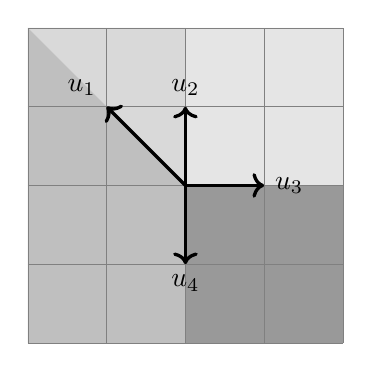
\begin{tikzpicture}
\path [fill=black!10!white] (0,0) -- (2,0) -- (2,2) -- (0,2) -- (0,0);
\path [fill=black!15!white] (0,0) -- (-2,2) -- (0,2) -- (0,0);
\path [fill=black!25!white] (0,0) -- (-2,2) -- (-2,-2) -- (0,-2) -- (0,0);
\path [fill=black!40!white] (0,0) -- (0,-2) -- (2,-2) -- (2,0) -- (0,0);
\draw [help lines] (-2,-2) grid (2,2);
\draw [->,very thick] (0,0) -- (-1,1) node[above left]{$u_1$};
\draw [->,very thick] (0,0) -- (0,1) node[above]{$u_2$};
\draw [->,very thick] (0,0) -- (1,0) node[right]{$u_3$};
\draw [->,very thick] (0,0) -- (0,-1) node[below]{$u_4$};
\end{tikzpicture}
\caption{Toric fan for $\mathbb F_1$.}
\end{figure}

\begin{figure}
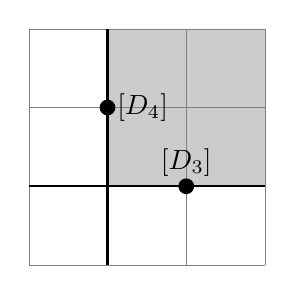
\begin{tikzpicture}
\path [fill=black!20!white] (0,0) -- (2,0) -- (2,2) -- (0,2) -- (0,0);
\draw [help lines] (-1,-1) grid (2,2);
\fill [black] (0,1) circle[radius=.1] node[right]{${[D_4]}$};
\fill [black] (1,0) circle[radius=.1] node[above]{${[D_3]}$};
\draw [thick] (-1,0) -- (2,0);
\draw [thick] (0,-1) -- (0,2);
\end{tikzpicture}
\caption{Nef cone $\operatorname{Nef}(\mathbb F_1)$.}
\end{figure}

\begin{figure}
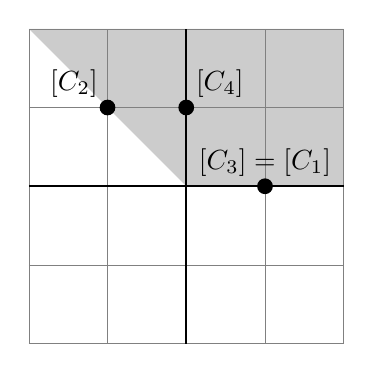
\begin{tikzpicture}
\path [fill=black!20!white] (0,0) -- (2,0) -- (2,2) -- (-2,2) -- (0,0);
\draw [help lines] (-2,-2) grid (2,2);
\fill [black] (0,1) circle[radius=.1] node[above right]{${[C_4]}$};
\fill [black] (1,0) circle[radius=.1] node[above]{${[C_3]}={[C_1]}$};
\fill [black] (-1,1) circle[radius=.1] node[above left]{${[C_2]}$};
\draw [thick] (-2,0) -- (2,0);
\draw [thick] (0,-2) -- (0,2);
\end{tikzpicture}
\caption{Mori cone $\overline{\operatorname{NE}}(\mathbb F_1)$.}
\end{figure}

$\Pic(\mathbb F_1)$ is generated by $[D_3]$ and $[D_4]$, with relations $[D_1]=[D_3]$ and $[D_2]=[D_4]-[D_3]$, and the intersection table is given by
\[
{}
\begin{cases}
 D_3^2=0 \\
 D_3.D_4=0 \\
 D_4^2=1
\end{cases} 
\]
When thinking of $\mathbb F_1$ as a $\PP^1$-bundle over $\PP^1$, $C_1$ and $C_3$ represent the fibers of the bundle (over the toric points of $\PP^1$), while $C_4$ (resp. $C_2$) is the zero/positive (resp. infinity/negative) section; when thinking of $\mathbb F_1$ as $\operatorname{Bl}_{p}\PP^1$, $C_2$ is the exceptional divisor, $C_4$ is the toric line not passing through $p$, and $C_1,C_3$ are the strict transforms of the toric lines through $p$.

Let us look at $\M{0}{2}{\mathbb F_1}{[C_4]}$. Since $[C_4]=[C_2]+[C_3]$, there are going to be maps of the following sort: the source curve is reducible $R_1\sqcup_q R_2$, $R_1$ is mapped isomorphically to a fiber (i.e. in class $[C_3]$) and $R_2$ is mapped isomorphically to $C_2$, all the markings belong to $R_1$. So $R_2$ is a rational tail and deserves to be contracted. Notice that the line bundle $\mathcal O(D_2)$ has degree $-1$ on $R_2$ (and $1$ on $R_1$). In this case everything works well because the corresponding section $u_{2|R_1}$ must vanish at the node, so we can divide it by a chosen (once for all toric line bundles) section of $\mathcal O_{R_1}(q)$.

Consider now $\M{0}{2}{\mathbb F_1}{2[C_2]+[C_3]}$. Certainly there are going to be maps similar to the ones described above, with $R_2$ now covering $C_2$ $2\colon 1$. The point is that $\mathcal O(D_2)$ has degree $-2$ on $R_2$, but $u_{2|R_1}$ doesn't have to vanish at the node of order $2$, so we are in trouble. \textcolor{blue}{Something is going on here: in this case there is a boundary component where the map is of the type that we have just described, and the requirement that $u_{2|R_1}$ vanishes of order $2$ at the node defines precisely the intersection with the main component. Check this. Could we possibly exploit this phenomenon to define a smaller compactification, possibly even smaller than quasimaps?}
\newpage

\section{Quasimap String Equation for $\PP^r$}

The string equation for the Gromov--Witten invariants of a smooth projective variety $X$ is given by
\begin{align*} \langle \mathbbm{1} , \gamma_1 \psi^{a_1} , \ldots, & \gamma_n \psi^{a_n} \rangle_{g,n+1,\beta}^X = \\
&  \sum_{i=1}^n \langle \gamma_1 \psi^{a_1}, \ldots, \gamma_{i-1} \psi^{a_{i-1}} , \gamma_i \psi^{a_i - 1} , \gamma_{i+1} \psi^{a_{i+1}} \ldots, \gamma_n \psi^{a_n} \rangle_{g,n,\beta}^X \end{align*}
where $\mathbbm{1} \in H^*(X)$ is the unit class (by convention any term involving a negative power of $\psi$ is set to zero). Since Gromov--Witten invariants and quasimap invariants coincide for $X=\PP^r$ (\cite[Section 5.4]{Manolache-Push}) we know that the same equation holds for quasimap invariants to $\PP^r$.

Nevertheless, it would be illuminating to have a direct proof of this statement, without relying on the equivalence with Gromov--Witten theory. Amongst other things, such a proof would necessarily involve some nontrivial intersection computations in the cohomology ring of the quasimap space, which would be of independent interest.

The proof of the classical string equation (for Gromov--Witten invariants) relies on three key lemmas involving certain codimension--1 classes on the moduli space of stable maps. Let
\begin{equation*} \pi : \M{g}{n+1}{X}{\beta} \to \M{g}{n}{X}{\beta}\end{equation*}
denote the contraction map given by forgetting the last marked point and stabilising. Then we have:

\begin{enumerate}
\item $\psi_i = \pi^* \psi_i + D_{i,n+1}$
\item $\psi_i \cdot D_{i,n+1} = 0$
\item $D_{i,n+1} \cdot D_{j,n+1} = 0$ for $i \neq j$
\end{enumerate}

Here $D_{i,n+1}$ is  the locus of stable maps $(C,x_1, \ldots, x_{n+1}, f)$ such that we can split up $C$ into two pieces, $C = C^\prime \cup C^{\prime\prime}$ (intersecting in a single node) such that $C^{\prime\prime}$ has degree $0$ and contains only the markings $x_i$ and $x_{n+1}$.

[FIGURE]

We would like to have some analogue of these results in the quasimap setting. In fact, equations (2) and (3) carry over without difficulty. Equation (1), on the other hand, is rather more delicate.

In the stable map setting, equation (1) is proved by considering the following diagram
\bcd
\mathcal{C}_{g,n+1} \ar[r,"\rho"] \ar[dr, "\psi" below left] & \pi^* \mathcal{C}_{g,n} \ar[r,"\alpha"] \ar[d, "\eta"] & \mathcal{C}_{g,n} \ar[d,"\varphi"] \\
& \M{g}{n+1}{X}{\beta} \ar[r,"\pi"] & \M{g}{n}{X}{\beta}
\ecd
where the square on the right is cartesian. On fibres, the map $\rho$ contracts rational components of $\mathcal{C}_{g,n+1}$ on which $f$ is constant and which contain exactly three special points, one of which is $x_{n+1}$. Thus, we see that
\begin{equation*} \rho^*(x_i) = x_i + R_{i,n+1} \end{equation*}
where $R_{i,n+1} \subseteq C_{g,n+1}$ consists fibrewise of the rational tails containing only $x_i$ and $x_{n+1}$; it is a closed substack of $\psi^{-1}(D_{i,n+1})$ of codimension $0$.

On the other hand, we have (REFERENCE):
\begin{equation*} \rho^* \omega_\eta(\Sigma_{i=1}^n x_i) = \omega_\psi(\Sigma_{i=1}^n x_i) \end{equation*}
Taking Chern classes and combining this with the above result we obtain:
\begin{equation*} \operatorname{c}_1(\rho^* \omega_\eta) = \operatorname{c}_1(\omega_\psi) - \Sigma_{i=1}^n R_{i,n+1} \end{equation*}
We can now pull back along the section $x_i$ and  use the fact that $x_i^* R_{j,n+1} = \delta_{i,j} D_{i,n+1}$ to obtain:
\begin{equation*} \operatorname{c}_1(x_i^*\rho^* \omega_\eta) = \operatorname{c}_1(x_i^* \omega_\psi) - D_{i,n+1} \end{equation*}
Now, $\rho^* \omega_\eta = \rho^* \alpha^* \omega_\varphi$, and so:
\begin{equation*} x_i^* \rho^* \omega_\eta = \pi^* x_i^* \omega_\varphi \end{equation*}
Thus we end up with
\begin{equation*} \pi^*\operatorname{c}_1(x_i^* \omega_\varphi) = \operatorname{c}_1(x_i^* \omega_\psi) - D_{i,n+1} \end{equation*}
which is equation (1) above.

What is different in the case of quasimaps? We have a similar-looking diagram
\bcd
\mathcal{C}_{g,n+1} \ar[r,"\rho"] \ar[dr, "\psi" below left] & \pi^* \mathcal{C}_{g,n} \ar[r,"\alpha"] \ar[d, "\eta"] & \mathcal{C}_{g,n} \ar[d,"\varphi"] \\
& \Q{g}{n+1}{X}{\beta} \ar[r,"\pi"] & \Q{g}{n}{X}{\beta}
\ecd
but now, because of the stronger stability condition, $\rho$ also contracts the locus $T_{n+1}$ consisting of rational tails (of any degree) with a single marking $x_{n+1}$. We claim that:

\begin{conj} $\rho^* \omega_\eta ( \Sigma_{i=1}^n x_i ) = \omega_\psi (\Sigma_{i=1}^n x_i - T_{n+1})$ \end{conj}

Once we have this, the string equation follows as in the stable maps case by pulling back along the section $x_i$ (and using the obvious fact that $x_i^* T_{n+1} = 0$).

\newpage
























\section{Quasimaps to $\PP^r$ relative to a hyperplane}

We first deal with genus 0 quasimaps to projective space, relative to a hyperplane. We give a Gathmann-like description of the space of relative quasimaps as a closed substack of the moduli space of (absolute) quasimaps to $\PP^r$; it turns out to be irreducible of the expected dimension. Finally, we retrieve a Gathmann-type formula by pushforward along the comparison morphism $\comp\colon \M{0}{n}{\PP^r}{d}\to\Q{0}{n}{\PP^r}{d}$.

Fix coordinates on $\PP^r$ such that the hyperplane $H$ is $\{x_0=0\}$. Let $\alpha=(\alpha_1,\ldots,\alpha_n)$ be an $n$-tuple of nonnegative integers. Consider the following locus $\Qt{0}{\alpha}{\PP^r|H}{d}$ inside $\Q{0}{n}{\PP^r}{d}$: the quasimaps $(C,x_1,\ldots,x_n,L,u_0,\ldots,u_r)$ such that, if $Z$ is a connected component of the vanishing locus of $u_0$ in $C$, then one of the following holds:

\begin{enumerate}
\item $Z$ is a point, either unmarked, or one of the $x_i$'s, and in this case $u_0$ vanishes at $Z$ with multiplicity at least $\alpha_i$.
\item $Z$ is a curve (\emph{internal}); letting $C^{(1)},\ldots,C^{(k)}$ be the (\emph{external}) irreducible components adjacent to $Z$, with nodes $q_i=Z\cap C^{(i)}$, and $m^{(i)}$ the order of vanishing of $u_{0|C^{(i)}}$ at $q_i$, we must have
\[
\deg(L_{|Z})+\sum_{i=1}^k m^{(i)}\geq\sum_{x_j\in Z} \alpha_j
\]
\end{enumerate}

On the other hand, denote by $\mathcal Q_{0,\alpha}(\PP^r|H,d)$ the \emph{nice locus}, consisting of actual maps from an irreducible curve (i.e. $\PP^1$) and with specified tangency condition $\alpha$ at the markings $\mathbf x$. Notice that this is an irreducible, locally closed substack of $\Q{0}{n}{\PP^r}{d}$, by pretty much the same argument as in \cite[Lemma 1.8]{Ga}; it has codimension $\sum\alpha$. In fact it is isomorphic to the nice locus inside stable maps, that Gathmann denotes by $\mathcal M_{0,\alpha}(\PP^r|H,d)$ \cite[Def. 1.6]{Ga} (the stricter stability condition has no effect when the source curve is irreducible, of course provided $n\geq2$); hence:

\begin{lem}\label{lem:comparison}
The comparison morphism restricts to a birational morphism $\M{0}{\alpha}{\PP^r|H}{d}\to \Qt{0}{\alpha}{\PP^r|H}{d}$.
\end{lem}
\begin{proof}
The contraction of a rational tail $R$ always happens far away from the markings, hence the only care we need to take is when the one component touching $R$ is internal (call it $Z$); in this case, observe that $m^{(R)}\leq\deg(f_{|R})$ and the quasimap resulting from the contraction of $R$ has $\deg(L_{|Z})=\deg(f_{|Z})+\deg(f_{|R})$, so the corresponding term only moves around the LHS of the $\alpha$-tangency condition nr. 2.

Birationality follows from the fact that the comparison morphism restricts to give an isomorphism between the nice loci.
\end{proof}

\begin{lem}
With notations as above (with $\sum\alpha\leq d$), $\Qt{0}{\alpha}{\PP^r|H}{d}$ is the closure of the nice locus $\mathcal Q_{0,\alpha}(\PP^r|H,d)$ inside $\Q{0}{n}{\PP^r}{d}$. 
\end{lem}
\begin{proof}
$\Qt{0}{\alpha}{\PP^r|H}{d}\subseteq\overline{\mathcal Q_{0,\alpha}(\PP^r|H,d)}$: we show that, given any quasimap satisfying the $\alpha$-tangency conditions spelled above, it can be (infinitesimally) deformed to a stable \emph{map} satisfying Gathmann's conditions \cite[Def. 1.1 and Rmk. 1.4]{Ga}, and then appeal to \cite[Prop. 1.14]{Ga}.

We induct on the number of components containing at least one base-point. If this number is zero, we're done (because quasimap stability is stronger than map stability); otherwise, pick such a component $C_0$, with base-points $p_1,\ldots,p_h$ and adjacent rational trees $R_1,\ldots,R_k$, joined to $C_0$ at the nodes $q_1,\ldots,q_k$. Since there are base-points but the quasimap respects the nondegeneracy condition, $\deg(L_{|C_0})>0$, and since $C_0\simeq\PP^1$ we can find a section $w$ of $L_{|C_0}\simeq\mathcal O_{\PP^1}(d_0)$ not vanishing at any of the base-points $p_i$'s; then it is enough to deform the section $u_{r|C_0}$ to $u_{r|C_0}+\epsilon w$ (and keep the other sections the same) in order to delete the base-points belonging to $C_0$. Notice that $u_{0|C_0}$ is unchanged, so the deformation still respects $\alpha$-tangency at the markings lying on $C_0$ (whether the latter is an internal or an external component). We need to check that such a deformation can be extended to the whole curve $C$ without changing the vanishing conditions on $u_0$. Notice that the action of $PGL_{r+1}$ on $\PP^r$ extends to an action of the group on the space of quasimaps; we can apply the matrix
\[
\begin{bmatrix}
1 & & \\
 & \ddots & \\
 & \epsilon \frac{w(q_i)}{u_j(q_i)} & 1
\end{bmatrix}
\]
to the restriction of the original quasimap to $R_i$, where $j$ is any index s.t. $u_j(q_i)\neq 0$ (one such must exist because the node is not allowed to be a base-point), and by doing this separately to every rational tree springing from $C_0$ we get a deformation of the original quasimap that still has $\alpha$-tangency with the hyperplane $H$ ($u_0$ hasn't been touched at all), but the base-points on $C_0$ have been eliminated.

$\overline{\mathcal Q_{0,\alpha}(\PP^r|H,d)}\subseteq\Qt{0}{\alpha}{\PP^r|H}{d}$: consider a family of relative quasimaps over a smooth curve $S$, such that the generic fiber lies in the nice locus. Then we may blow-up the source curve (which is a fibered surface) in the base-points of the quasimap (that are finitely many smooth points of the central fiber) in order to get an actual morphism to $\mathbb P^r$; we may as well suppose that the central fiber of the new family is stable. Notice that the central fiber actually belongs to Gathmann's space $\M{0}{\alpha}{\PP^r|H}{d}$: we have just introduced some rational tails away from the markings, hence the only thing we have to check is, when we blow-up a base-point on an internal component, the rational tail will again be internal ($u_0\equiv 0$ in a neighborhood of the base-point), so it will contribute to the LHS of the $\alpha$-tangency condition nr. 2 in the very same way. We may now invoke \cite[Lemma 1.9]{Ga} and the quasimap case follows from Lemma \ref{lem:comparison}.
\end{proof}
From now on we shall denote this closed substack by $\Q{0}{\alpha}{\PP^r|H}{d}$.

\medskip

Increasing the multiplicity can be naively performed in the very same way as Gathmann did:
\[
\sigma^m_k:=x_k^*d^m_{\mathcal C/\overline{\mathcal Q}}(u_0)\in H^0(\overline{\mathcal Q},x_k^*\mathcal P^m_{\mathcal C/\overline{\mathcal Q}}(\mathcal L))
\]
with $m=\alpha_k+1$ cuts $\Q{0}{\alpha+e_k}{\PP^r|H}{d}$ inside $\Q{0}{\alpha}{\PP^r|H}{d}$, together with a bunch of degenerate contributions from quasimaps where the component on which $x_k$ lies is internal (call it $Z$) and (notice the equality sign!)
\[
\deg(L_{|Z})+\sum m^{(i)}=\sum_{x_j\in Z}\alpha_j.
\]
Of course, quasimap stability forces these degenerate contributions not to have any rational tail; this is really the only difference with the case of stable maps, and indeed we can pushforward Gathmann's formula along the comparison morphism $\comp\colon \M{0}{n}{\PP^r}{d}\to\Q{0}{n}{\PP^r}{d}$ and the only terms that are going to change are the degenerate ones with rational tails (in fact they disappear, since the restriction of the comparison map has positive dimensional fibers there). With an eye to the future, we remark that these contributions do matter when computing GW invariants of a CY hypersurface in projective space, and may well account for the divergence between GW and quasimap invariants in the CY case \cite[Rmk. 1.6]{Ga-MF}.

\begin{lem}\label{lem:compare_psi}
$\comp^*(\psi_k)=\psi_k$ and $\comp^*(x_k^*\mathcal L)=\ev_k^*(\mathcal O_{\mathbb P^r}(H))$.
\end{lem}
\begin{proof}
Recall that $\psi_k=c_1(x_k^*\omega_{\mathcal C/\mathcal M})$ and contemplate the following diagram
\bcd
& & & \PP^r & \\
\mathcal C_{\overline {\mathcal M}}\ar[rr,"\sst"]\ar[rd] \ar[urrr,"f"] & & \comp^*\mathcal C_{\overline {\mathcal Q}} \ar[ld]\ar[rr]\ar[ur,dashed] & & \mathcal C_{\overline {\mathcal Q}} \ar[d]\ar[ul,dashed] \\
& \M{0}{n}{\PP^r}{d} \ar[rrr,"\comp"] \ar[ul,bend left,"x_k"]\ar[ur,bend right,"x_k"right=.2cm]& & & \Q{0}{n}{\PP^r}{d}\ar[u,bend right, "x_k"right]
\ecd
where $\sst$ is the strong stabilisation map, i.e. contracting the rational tails, which is an isomorphism near the markings.
\end{proof}

\begin{lem}\label{lem:posdimfiber}
$\dim(\M{0}{(m^{(i)})}{\PP^r|H}{d}\cap \ev_1^*(p))>0$ everytime $rd>1$, where $p$ is a point of $H$, so the pushforward along $\comp$ of a degenerate locus with rational tails is 0.
\end{lem}
\begin{proof}
$\dim(\M{0}{(m^{(i)})}{\PP^r|H}{d}\cap \ev_1^*(p))=(r-3)+(1-m^{(i)})+d(r+1)-(r-1)=(rd-1)+(d-m^{(i)})$.
\end{proof}

\begin{prop}
Denote by $[D^\mathcal{Q}_{\alpha,k}(\PP^r|H,d)]$ the sum of the (product) fundamental classes of
\[
\Q{0}{\alpha^{(0)}\cup {(0,\ldots,0)}}{H}{d_0}\times_{(\PP^r)^k}\prod_{i=1}^k \Q{0}{(m^{(i)})\cup\alpha^{(i)}}{\PP^r|H}{d_i}
\]
with coefficient $\frac{m^{(1)}\ldots m^{(k)}}{k!}$, where the sum runs over all splittings $d=\sum d_i$ and $\alpha=\bigcup \alpha^{(i)}$ such that the above spaces are well-defined, in particular $|\alpha^{(0)}|+k$ and $|\alpha^{(i)}|+1$ are all $\geq 2$, and such that
\[
d_0+\sum_{i=1}^k m^{(i)}=\sum \alpha^{(0)}
\]

The following formula holds
\[
(\alpha_k\psi_k+x_k^*\mathcal L)\cdot[\Q{0}{\alpha}{\PP^r|H}{d}]=[\Q{0}{\alpha+e_k}{\PP^r|H}{d}]+[D^\mathcal{Q}_{\alpha,k}(\PP^r|H,d)].
\]
\end{prop}
\begin{proof}
Follows from \cite[Thm. 2.6]{Ga} by pushforward along $\comp\colon \M{0}{n}{\PP^r}{d}\to\Q{0}{n}{\PP^r}{d}$, using the projection fomula and Lemmas \ref{lem:comparison}, \ref{lem:compare_psi} and \ref{lem:posdimfiber}.
\end{proof}

\section{Comparison with the GIT construction}
Let $X$ be a hypersurface of degree $a$ in $\PP^r$. In the preceding sections, we have put a virtual class on $\Q{g}{n}{X}{d}$ by way of the following Cartesian diagram:

\bcd
\Q{g}{n}{X}{d}\ar[d]\ar[r] & \Q{g}{n}{\PP^r}{d}\ar[d,"\nu_a"] \\
\Q{g}{n}{H}{ad}\ar[r] & \Q{g}{n}{\PP^N}{ad}
\ecd

where $N={{r+a}\choose{a}}-1$ and $\nu_a$ is the Veronese embedding. In fact, $\Q{g}{n}{X}{d}$ is thought of as representing stable quasimaps to $\PP^r$ such that the corresponding sections satisfy the equation for $X$ inside $\PP^r$, that is a homogeneous polynomial $Q$ of degree $a$, i.e. gives a section of $L^{\otimes a}$ on the source curve $C$.

We wish to compare this with the GIT approach of \cite{CFKM}. Here $X$ is seen as the GIT quotient of the affine cone $C_X\subseteq \mathbb A^{r+1}$ with respect to the diagonal $\mathbb G_m$-action. Objects of $\Q{g}{n}{X}{d}^\text{GIT}$ are diagrams of the form

\bcd
P\ar[d,"\mathbb G_m"]\ar[r] & C_X & \text{or, equivalently,} & P\times_{\mathbb G_m} C_X \ar[d,"\rho" left] \\
C & & & C \ar[u,bend right,"u"right]
\ecd
and the dual perfect obstruction theory with respect to $\mathfrak{Bun}_{\mathbb G_m}$ is given by $R^\bullet\pi_*(u^*\mathbb T^\bullet_\rho$), where $\pi\colon \mathcal C_{\mathfrak{Bun}}\to\mathfrak{Bun}_{\mathbb G_m}$ is the universal curve.

Notice that $\mathfrak{Bun}_{\mathbb G_m}\simeq \mathfrak{Pic}$ by taking the line bundle $L=P\times_{\mathbb G_m}\mathbb A^1\to C$ associated to the $\mathbb G_m$-torsor $P\to C$. Furthermore, the $\mathbb G_m$-equivariant embedding in a smooth stack
\bcd
P\times_{\mathbb G_m} C_X \ar[r,hook]\ar[d,"\rho" left] & P\times_{\mathbb G_m}\mathbb A^{r+1}\simeq L^{\oplus r+1}\ar[dl]\\
C \ar[u,bend right,"u"right] &
\ecd
gives us $u^*T^\bullet_\rho\simeq[L^{\oplus r+1}\to L^{\otimes a}]$, where the arrow is induced by $Q$, and shows that both the modular interpretation and the obstruction theory coincide.

\section{The quasimap mirror theorem}
Assuming that quasimap invariants for $\PP^r$ coincide with Gromov-Witten invariants on the nose, we get the following result.
\begin{dfn}
 For a complete intersection $X$ in $\PP^r$ and $d>0$, let
 \[
  I^X_d=(\ev_1)_*\left(\frac{1}{z-\psi_1}[\Q{0}{2}{X}{d}]^\text{vir}\right)
 \]
 where $\ev_1$ is always thought of as landing in $\PP^r$.
 
 Set also $I^X_0=\mathbbm 1_{\PP^r}$ and $I^X=\sum_{d\geq 0}I^X_d q^d$.
\end{dfn}
\begin{thm}
Let $X\subseteq\PP^4$ be a smooth quintic 3-fold. Then
 \[
  \sum_{d\geq 0} q^d\prod_{i=0}^{5d}(X+iz)I^{\PP^4}_d= XP(q)I^X
 \]
where
\[
 P(q)=1+\sum_{d>0}dq^d\langle H^4,\mathbbm 1_{\PP^4}\rangle_{\Q{0}{\{5d,0\}}{\PP^4|X}{d}}=1+\sum_{d>0}q^d\frac{(5d)!}{(d!)^5}\sum_{i=d+1}^{5d-1}\frac{1}{i}.
\]
\end{thm}
\begin{proof}
 We'll write it for a general CY hypersurface in $i\colon X_a\hookrightarrow\PP^r$, so the degree of $X$ is $a=r+1$. Notice that dual bases for $H^*(\PP^r)$ are given by $T^i=H^i$ and $T_i=H^{r-i}$, while (induced) dual bases for $i^*H^*(\PP^r)$ are $S^i=H^i$ and $S_i=\frac{1}{a}H^{r-i-1}$; the restriction of $H^r$ is 0.
 
 Define
 \[
  I^{\PP^r|X}_{d,(m)}=(\ev_1)_*\left(\frac{1}{z-\psi_1}[\Q{0}{\{m,0\}}{\PP^r|X}{d}]^\text{vir}\right),
 \]
which coincides with the absolute $I$-function defined above for $m=0$, and
\[
 J^{\PP^r|X}_{d,(m)}=(\ev_1)_*\left(m[\Q{0}{\{m,0\}}{\PP^r|X}{d}]^\text{vir}+\frac{1}{z-\psi_1}[D_m^{\mathcal Q}(\PP^r|X,d)]^\text{vir}\right).
\]
Then, by Gathmann's formula, we can prove that
\begin{equation}\label{eqn:G}
 (X+mz) I^{\PP^r|X}_{d,(m)}= I^{\PP^r|X}_{d,(m+1)}+ J^{\PP^r|X}_{d,(m)},
\end{equation}
from which it follows that
\[
 \prod_{i=0}^{ad}(X+iz) I^{\PP^r}_d=\sum_{m=0}^{ad}\prod_{i=m+1}^{ad}(X+iz)J^{\PP^r|X}_{d,(m)}.
\]
It is now a matter of evaluating the RHS. Notice that $J^{\PP^r|X}_{d,(m)}$ is made of two parts:
\begin{itemize}
 \item the boundary terms: the strong stability condition for quasimaps and the choice of working with only two markings makes these boundary contributions particularly simple to compute. The shape of the source curve is that of a snake which the hypersurface cuts into two pieces, the internal one of degree $d^{(0)}$, and the external one of degree $d^{(1)}$ and multiplicity $m^{(1)}$ of contact with $X$, with the first marking point belonging to the internal component and the second to the external one.
 
 The invariants which we need to consider will hence be of the form
 \[
  \langle T^i\psi_1^j,S_i\rangle_{\Q{0}{2}{X}{d^{(0)}}}\langle S^i,\mathbbm 1_{\PP^r}\rangle_{\Q{0}{\{m^{(1)},0\}}{\PP^r|X}.{d^{(1)}}}
 \]
 A dimensional computation
\begin{align*}
 0\leq \codim S_i &= \dim X-\codim S^i \\
 &= \dim X-\vdim \Q{0}{\{m^{(1)},0\}}{\PP^r|X}{d^{(1)}} \\
 &= \dim X-(\dim\PP^r-3+2-m^{(1)}-K_{\PP^r}\cdot d^{(1)}\ell)\\
 &= m^{(1)}-X\cdot d^{(1)}\ell+K_{X}\cdot d^{(1)}\ell \\
 &= m^{(1)}-X\cdot d^{(1)}\ell\leq 0
\end{align*}
forces $S_1=\mathbbm 1_X$ and $S^1=\frac{1}{a}H^{r-1}$, $m^{(1)}=ad^{(1)}$ hence
\[
 m=\alpha_1=X\cdot d^{(0)}\ell+m^{(1)}=ad,
\]
so this doesn't show up but at the very end of the ``increasing the multiplicity'' process.

\item The other term in $J^{\PP^r|X}_{d,(m)}$ is $m(\ev_1)_*[\Q{0}{\{m,0\}}{\PP^r|X}{d}]^\text{vir}$; notice that it only gets insertions from the cohomology of $\PP^r$ (restricted to $X$). On the other hand
\[
 \vdim \Q{0}{\{m,0\}}{\PP^r|X}{d}=r-3+2-m+d(r+1)\geq r-1
\]
because $m\leq ad$; since the restriction of $H^r$ to $X$ vanishes, the only insertion that contributes is $H^{r-1}$, forcing the equality $m=ad$.
\end{itemize}
So, in the end, we see that equation \ref{eqn:G} reduces to
\begin{align*}
 \prod_{i=0}^{ad}(X+iz) I^{\PP^r}_d &=J^{\PP^r|X}_{d,(ad)} \\
 &= \sum_{i=0,\ldots,r-1;j\geq 0}(da)\langle H^{r-1},\mathbbm 1_{\PP^r}\rangle_{\Q{0}{\{ad,0\}}{\PP^r|X}{d}} H \\
 &+\sum_{\substack{0<d^{(0)}<d \\ d^{(0)}+d^{(1)}=d}}z^{j+1}H^{r-i}\langle H^i\psi_1^j,\mathbbm 1_{X}\rangle_{\Q{0}{2}{X}{d^{(0)}}}(ad^{(1)})\langle \frac{1}{a}H^{r-1},\mathbbm 1_{\PP^r}\rangle_{\Q{0}{\{ad^{(1)},0\}}{\PP^r|X}{d^{(1)}}}\\
 &+z^{j+1}H^{r-i}\langle H^i\psi_1^j,\mathbbm 1_{X}\rangle_{\Q{0}{2}{X}{d}}
\end{align*}
from which the first claim of the theorem is now evident (with a bit of rearranging, using $X=aH$ and $i^*(H^r)=0$, so in the last line everything is divisible by $H$).

\smallskip

In order to evaluate $P(q)$, we use again Gathmann's algorithm, this time in the other direction, to go all the way back to $\PP^r$; then we make use of our assumption that quasimap invariants and ordinary GW coincide for the projective space. So it starts:
\[
 [\Q{0}{\{ad,0\}}{\PP^r|X}{d}]^\text{vir}=(X+(ad-1)\psi_1)[\Q{0}{\{ad-1,0\}}{\PP^r|X}{d}]^\text{vir}-[D_{ad}^{\mathcal Q}(\PP^r|X,d)]^\text{vir}
\]
When looking at the boundary, the invariants that come into play are of the form
\[
 \langle H^{r-1},S_i\rangle_{\Q{0}{2}{X}{d^{(0)}}}\langle S^i,\mathbbm 1_{\PP^r}\rangle_{\Q{0}{\{a(d-d^{(0)})-1,0\}}{\PP^r|X}{d-d^{(0)}}}
\]
but notice that they must vanish by dimensional reasons, since
\[
 \codim(S_i)=\dim X-3+2-K_X\cdot d^{(0)}\ell-(r-1)=-1.
\]
So
\begin{align*}
 d\langle H^{r-1},\mathbbm 1_{\PP^r}\rangle_{\Q{0}{\{ad,0\}}{\PP^r|X}{d}} \\
 = d[\Q{0}{2}{\PP^r}{d}]\cap\ev_1^*(H^{r-1})\prod_{i=0}^{ad-1}(\ev_1^*X+i\psi_1) \\
 = d[\Q{0}{2}{\PP^r}{d}]\cap\left((da-1)!\psi_1^{ad}\ev_1^*(H^{r-1})+a\left(\sum_{j=1}^{ad-1}\frac{(ad-1)!}{j}\right)\psi_1^{ad-1}\ev_1^*(H^{r})\right) \\
 = d\left((da-1)!\langle \psi_1^{ad-1}H^{r-1}\rangle_{0,1,d}+a\left(\sum_{j=1}^{ad-1}\frac{(ad-1)!}{j}\right)\langle\psi_1^{ad-2}H^{r}\rangle_{0,1,d}\right)
\end{align*}
using the equality of quasimap and GW invariants and the string equation for the latter. These numbers can be extracted from the $J$-function for $\PP^r$
\[
 I^{\PP^r}_d=\prod_{i=1}^d\frac{1}{H+i}
\]
from which
\begin{align*}
 \langle \psi_1^{ad-2}\ev_1^*(H^{r})\rangle_{0,1,d} &=\frac{1}{(d!)^{r+1}} \\
 \langle \psi_1^{ad-1}\ev_1^*(H^{r-1}\rangle_{0,1,d} &=-(r+1)\frac{1}{(d!)^{r+1}}\sum_{j=1}^d\frac{1}{j}
\end{align*}
and the second claim of the theorem follows.
\end{proof}

\bibliographystyle{alpha}
\bibliography{relqm}

\end{document}
